\section{Anwendungsbereiche}
\label{sec:usecases}
In diesem Abschnitt werden einige der aktuellen Anwendungsbereiche von WebGL vorgestellt.
Zu beachten ist, die Abbildungen sind logischwerweiße wieder nur 2D Bilder und können deshalb nicht die vollen Eindrücke der jeweiligen Seiten wiedergeben, dafür ist ein Besuch der Internetseite nötig.
\subsection{Google Maps}
Eine der wohl bekanntesten Beispiele wo WebGL angewendet wird ist Google Maps.
Hierbei profitiert die in Abbildung~\ref{fig:GoogleMaps} gezeigte Satellitenansicht von der dritten Dimension.
Gebäude können dadurch deutlich realitätsnaher dargestellt werden als auf einer einfachen Karte, auf der man nur die Umrisse sieht.
\begin{figure}
    \centering
    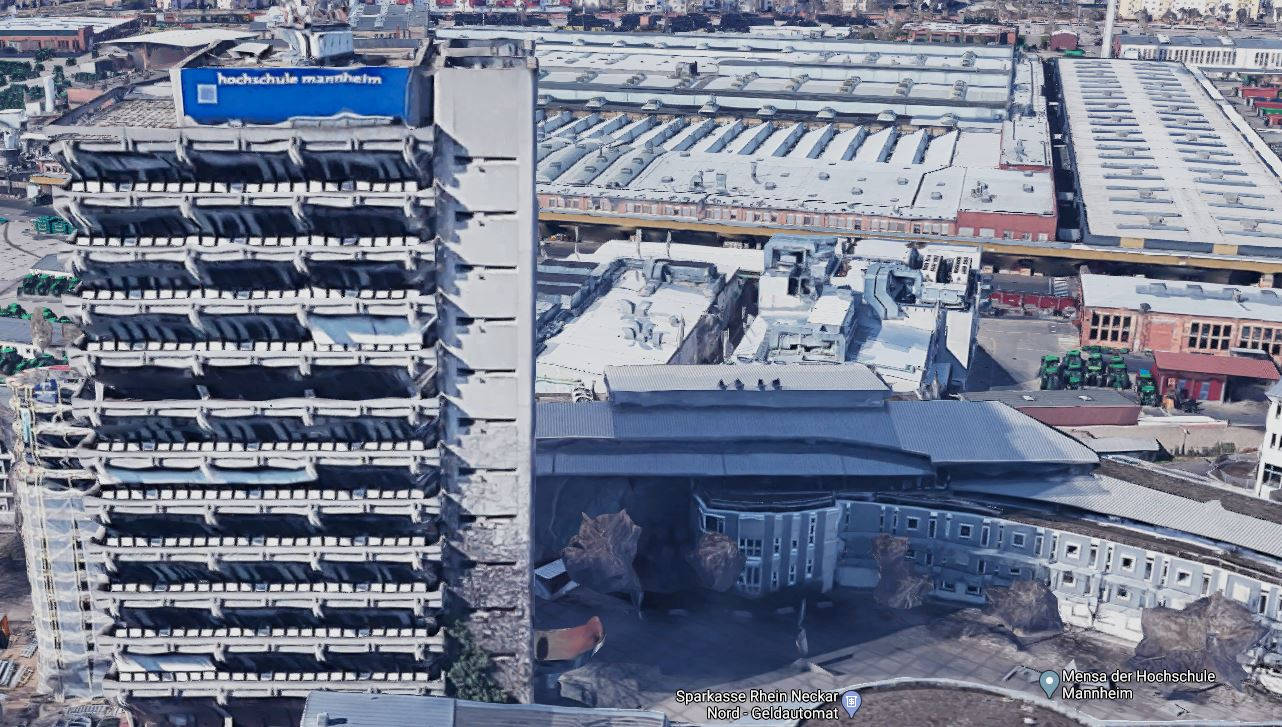
\includegraphics[width=6cm]{GoogleMapsExample.jpg}
    \caption{Google Maps Satellitenansicht \cite{GoogleMaps}} \label{fig:GoogleMaps}
    \end{figure}

\subsection{Online Shopping}
Online Shopping ist ein weiters Beispiel das zur heutigen Zeit fast ausschließlich 2 Dimensional stattfindet.
Durcch die fehlende dritte Dimension können Artikel etwas schlechter angesehen werden, die meisten Online Shopping Seiten versuchen dies durch das Anbieten von Fotos aus verschiedenen Perspektiven zu lösen.
Durch WebGL entsteht die Möglichkeit dies in wirklichem 3D darzustellen, als Beispiel hierfür wurde die Seite Hypebeast gewählt, diese stellt zum Beispiel einen Adidas Schuh auf moderne Art vor, zuerst erhält man eine virtuelle Reise auf der man viele Informationen zu dem besagten Schuh erhält, danach kann man diesen Schuh in 3D anschauen, drehen und die verschiedenen Modelle auswählen was man in Abbildung~\ref{fig:HypeBeast} sehen kann.
\begin{figure}
    \centering
    \includegraphics[width=6cm]{Hypebeast.jpg}
    \caption{Hypebeast Ozweego Presentation \cite{hypbeast}} \label{fig:HypeBeast}
    \end{figure}

\subsection{3D Entwicklung und 3D Druck}
Ein weiterer Bereich in dem WebGL bereits sehr stark angewendet wird, ist die 3D Entwicklung und der 3D Druck. In beiden Bereichen wollen Leute 3D Modelle erstellen und diese an andere Leute Verkaufen.
Damit sich der Käufer die Modelle vor dem Kauf bereits komplett anschauen kann, wird auch hier WebGL verwendet. \cite{manuninja}
In Abbildung~\ref{fig:sketchfab} sieht man ein solches 3D Modell, man kann sich das Modell einfach so anschauen, drehen und vergrößern. Außerdem kann man sich dort auch spezielle Details wie die Knochenstruktur des Modells oder
die verwendete Materialien anschauen. Es ist schon fast genauso gut wie wen man das Modell gekauft und in einem 3D Modellierungsprogramm geöffnet hat. Des weiteren gibt es sogar Seiten die das eigentliche 3D Modellieren im Browser ermöglichen wie zum Beispiel SculptGL. \cite{sculptgl}
\begin{figure}
    \centering
    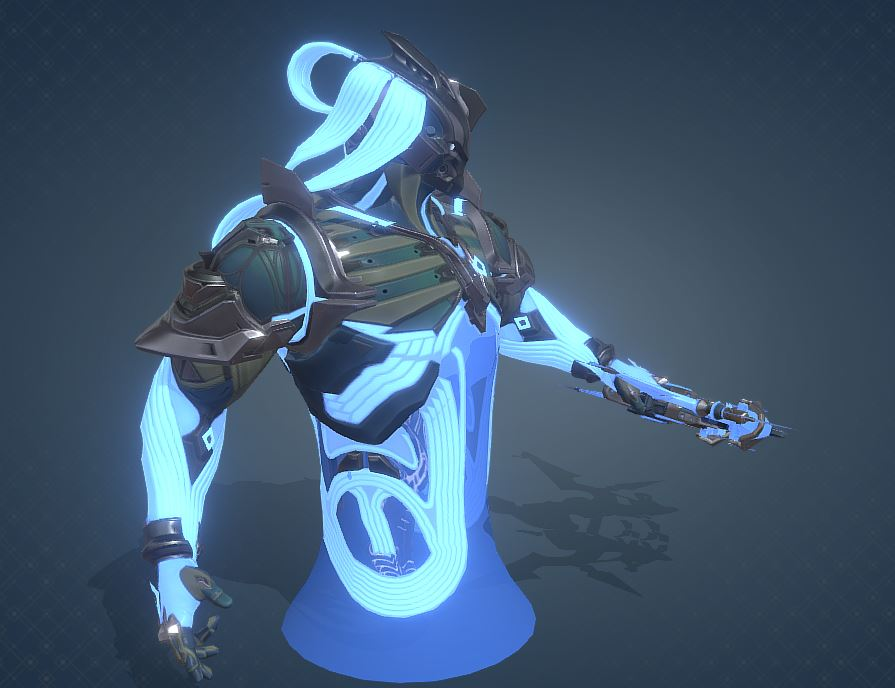
\includegraphics[width=6cm]{sketchfab.jpg}
    \caption{3D Modell Marktplatz \cite{sketchfab}} \label{fig:sketchfab}
    \end{figure}

\subsection{3D Simulationen im Bereich Medizin}
Auch in der Medizin findet WebGL viele Anwendungsbereiche, die Seite BioDigital ermöglicht das Simulieren und Darstellen des Menschlichen Körpers und vielen mehr.
In Abbildung~\ref{fig:BioDigital} sieht man die Simulation eines Menschlichen Körpers der COVID-19 Symptomen aufweißt, diese Simulationen können zur Weiterbildung im Medizinischen Umfeld, zum aufklären von Patienten und vielem mehr verwendet werden.\cite{BioDigital}
\begin{figure}
    \centering
    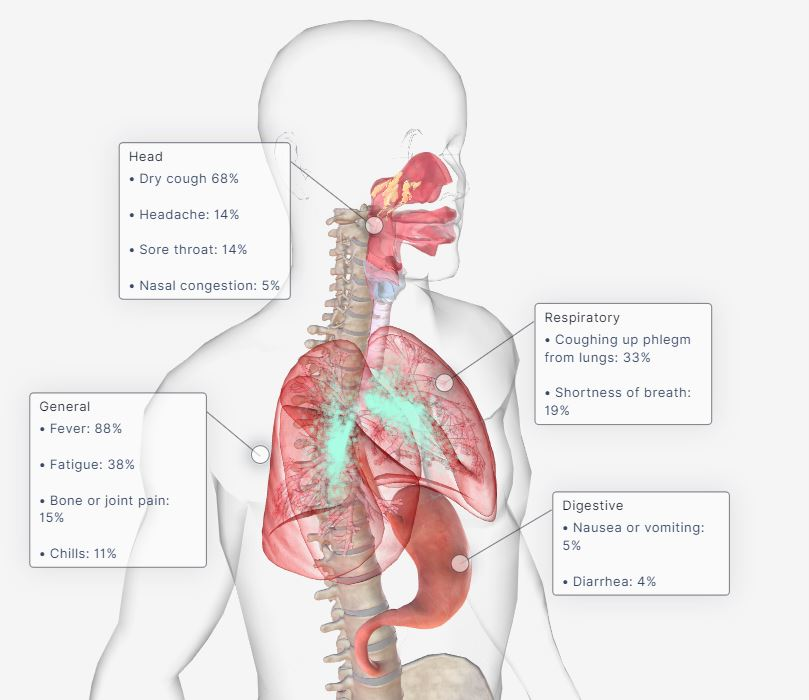
\includegraphics[width=6cm]{BioDigital.jpg}
    \caption{3D Simulation eines Körpers mit COVID-19 Symptomen \cite{BioDigital}} \label{fig:BioDigital}
    \end{figure}